% This file was created by tikzplotlib v0.9.1.
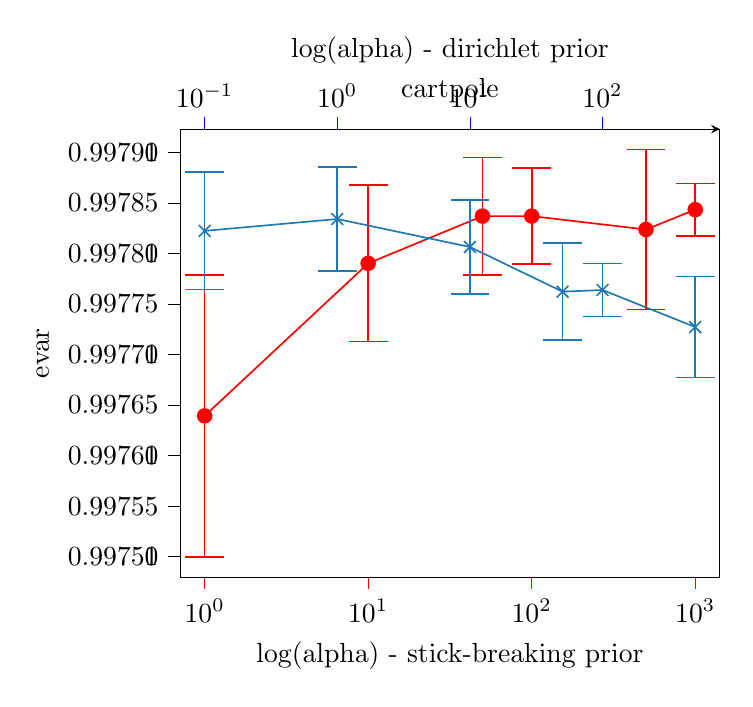
\begin{tikzpicture}

\definecolor{color0}{rgb}{0.12156862745098,0.466666666666667,0.705882352941177}

\begin{axis}[
log basis x={10},
tick align=outside,
tick pos=left,
title={cartpole},
x grid style={white!69.0196078431373!black},
xlabel={log(alpha) - stick-breaking prior},
xmin=0.707945784384138, xmax=1412.53754462275,
xmode=log,
xtick style={color=red},
xtick={0.01,0.1,1,10,100,1000,10000,100000},
xticklabels={\(\displaystyle {10^{-2}}\),\(\displaystyle {10^{-1}}\),\(\displaystyle {10^{0}}\),\(\displaystyle {10^{1}}\),\(\displaystyle {10^{2}}\),\(\displaystyle {10^{3}}\),\(\displaystyle {10^{4}}\),\(\displaystyle {10^{5}}\)},
y grid style={white!69.0196078431373!black},
ylabel={evar},
ymin=0.997479538637803, ymax=0.997922982589806,
ytick style={color=black},
ytick={0.99745,0.9975,0.99755,0.9976,0.99765,0.9977,0.99775,0.9978,0.99785,0.9979,0.99795},
yticklabels={0.99745,0.99750,0.99755,0.99760,0.99765,0.99770,0.99775,0.99780,0.99785,0.99790,0.99795}
]
\path [draw=red, semithick]
(axis cs:1,0.997499695181076)
--(axis cs:1,0.997778954281966);

\path [draw=red, semithick]
(axis cs:10,0.997712869162691)
--(axis cs:10,0.997867467410567);

\path [draw=red, semithick]
(axis cs:50,0.997778864379882)
--(axis cs:50,0.997894922135635);

\path [draw=red, semithick]
(axis cs:100,0.997789399158815)
--(axis cs:100,0.997884374880532);

\path [draw=red, semithick]
(axis cs:500,0.997744449062023)
--(axis cs:500,0.997902826046533);

\path [draw=red, semithick]
(axis cs:1000,0.997817383621656)
--(axis cs:1000,0.997869146071448);

\addplot [semithick, red, mark=-, mark size=7, mark options={solid}, only marks]
table {%
1 0.997499695181076
10 0.997712869162691
50 0.997778864379882
100 0.997789399158815
500 0.997744449062023
1000 0.997817383621656
};
\addplot [semithick, red, mark=-, mark size=7, mark options={solid}, only marks]
table {%
1 0.997778954281966
10 0.997867467410567
50 0.997894922135635
100 0.997884374880532
500 0.997902826046533
1000 0.997869146071448
};
\addplot [semithick, red, mark=*, mark size=2.5, mark options={solid}]
table {%
1 0.997639324731521
10 0.997790168286629
50 0.997836893257758
100 0.997836887019673
500 0.997823637554278
1000 0.997843264846552
};
\end{axis}

\begin{axis}[
axis x line=top,
log basis x={10},
tick align=outside,
x grid style={white!69.0196078431373!black},
xlabel={log(alpha) - dirichlet prior},
xmin=0.0653208007180445, xmax=765.452956031933,
xmode=log,
xtick pos=right,
xtick style={color=blue},
xtick={0.001,0.01,0.1,1,10,100,1000,10000},
xticklabels={\(\displaystyle {10^{-3}}\),\(\displaystyle {10^{-2}}\),\(\displaystyle {10^{-1}}\),\(\displaystyle {10^{0}}\),\(\displaystyle {10^{1}}\),\(\displaystyle {10^{2}}\),\(\displaystyle {10^{3}}\),\(\displaystyle {10^{4}}\)},
y grid style={white!69.0196078431373!black},
ymin=0.997479538637803, ymax=0.997922982589806,
ytick pos=left,
ytick style={color=black}
]
\path [draw=color0, semithick]
(axis cs:0.1,0.99776425060827)
--(axis cs:0.1,0.997880329693452);

\path [draw=color0, semithick]
(axis cs:1,0.997782469865019)
--(axis cs:1,0.997885559330014);

\path [draw=color0, semithick]
(axis cs:10,0.997759866211867)
--(axis cs:10,0.997852881603069);

\path [draw=color0, semithick]
(axis cs:50,0.997714093936285)
--(axis cs:50,0.997810152984651);

\path [draw=color0, semithick]
(axis cs:100,0.997737716315013)
--(axis cs:100,0.997789882056909);

\path [draw=color0, semithick]
(axis cs:500,0.99767715670559)
--(axis cs:500,0.997777097787524);

\addplot [semithick, color0, mark=-, mark size=7, mark options={solid}, only marks]
table {%
0.1 0.99776425060827
1 0.997782469865019
10 0.997759866211867
50 0.997714093936285
100 0.997737716315013
500 0.99767715670559
};
\addplot [semithick, color0, mark=-, mark size=7, mark options={solid}, only marks]
table {%
0.1 0.997880329693452
1 0.997885559330014
10 0.997852881603069
50 0.997810152984651
100 0.997789882056909
500 0.997777097787524
};
\addplot [semithick, color0, mark=x, mark size=3, mark options={solid}]
table {%
0.1 0.997822290150861
1 0.997834014597516
10 0.997806373907468
50 0.997762123460468
100 0.997763799185961
500 0.997727127246557
};
\end{axis}

\end{tikzpicture}
